\section{Linux Networking}
\label{sec:linuxNetworking}

Esta sección recopilará todos los conceptos y herramientas relacionadas con la parte de Networking en Linux, que son fundamentales para el desarrollo, análisis y validación de este proyecto.


%%%%%%%%%%%%%%%%%%%%%%%%%%%%%%%%%%%%%%%%%%%%%%%%%%%%%%%%%%%%%%%%%%%%%%%%%%%%%%%%%%%%%%%%%%

\subsection{Interfaz virtual - \texttt{tun/tap}}
\label{linuxNetworking_tuntap}

En el mundo de las redes siempre se habla de las interfaces tun/tap de forma indistinta cuando van a utilizarse, sin embargo, cada una tiene su cometido. Como se ha indicado, en networking, las interfaces TUN y TAP son interfaces virtuales que se crean y se gestionan en espacio de kernel. Mencionar que como estas interfaces son virtuales y se gestionan directamente vía softaware, no como las interfaces reales que se gestionan con unos drivers diferentes, cada interfaz con su driver específico de la interfaz.  Los drivers de las interfaces TUN/TAP se crearon en los 2000 como una unión de los avances de los drivers desarrollados en las comunidades de Solaris, Linux, BSD. Actualmente los drivers solo tienen mantenimiento por los kernels de linux y FreeBSD. Ambos tipos de interfaces se utilizan para tunelado, pero no pueden ser utilizadas a la vez dado que trabajan en niveles distintos. Las TUN, de \textit{network \textbf{TUN}nel}, emula la capa de red y puede llegar hacer reenvío de los paquetes. En cambio las interfaces TAP,  trabajan en capa 2 solo en capa dos, y emulan un equipo que trabaja en dicha capa, como por ejemplo un switch \cite{tuntap1}. Por tanto, hay que dejar claro lo que se puede llegar a realizar con cada interfaz (Ver figura \ref{fig:linux1}).

\begin{itemize}
    \item \texttt{TUN} se puede llegar a utilizar para routing.
    \item \texttt{TAP} se puede llegara utilizar para crear un bridge.
\end{itemize}

Generalmente, cuando los paquetes son enviados por el sistema operativo a través de una interfaz TUN/TAP,  serán recibidos por algún programa de espacio de usuario, el cual, está enganchado directamente en la interfaz. Cualquier programa de espacio de usuario podrá pasar paquetes por las interfaces, y las interfaces virtuales se lo pasarán al \textit{stack} de red por defecto, emulando la recepción de los paquetes inyectados desde espacio de usuario.

% fig
\begin{figure}[ht]
    \centering
    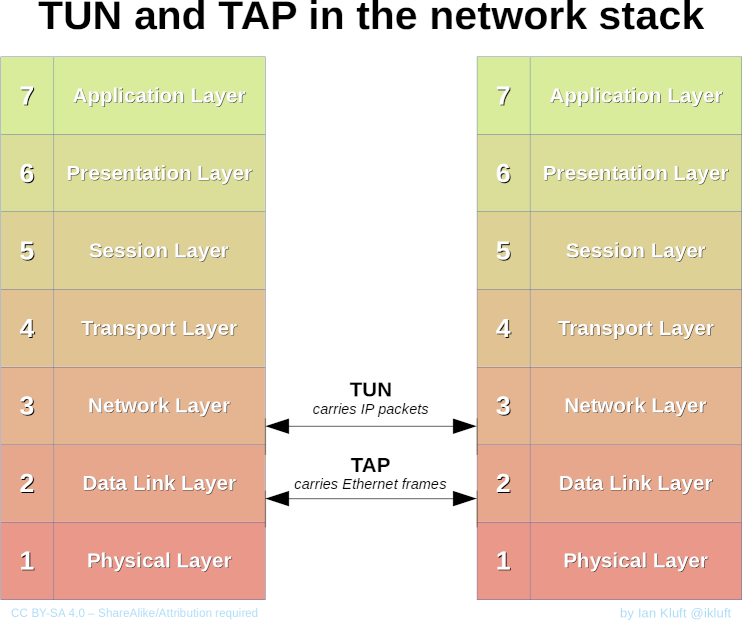
\includegraphics[width=\textwidth]{archivos/img/teoria/linux1.png}
    \caption{Diagrama de funcionamiento de las interfaces virtuales TUN/TAP \cite{tuntap2}}
    \label{fig:linux1}
\end{figure}

Para la creación de estas interfaces lo podemos hacer por ioctl o podemos hacerlo más fácil a través del binario tunctl o en su defecto con el comando de \texttt{tuntap} del set de herramientas iproute2. A continuación, en el bloque \ref{code:tun_tap_use} se indican todos los comandos necesarios para trabajar con las interfaces TUN/TAP.

\begin{lstlisting}[language= bash, style=Consola, caption={Manejo de interfaces TUN - TAP},label=code:tun_tap_use]
    # En caso de querer utilizar tunctl hay que instalar el binario
    sudo apt install -y uml-utilities
    
    # Para crear una un interfaz podemos hacer lo siguiente
    tunctl -t {nombre_tun}

    # Para eliminarla
    tunctl -d {nombre_tun}

    # Para crear interfaces de tipo TAP hay que hacer lo siguiente
    tunctl -p -t {nombre_tun}
    
    # El comando análogo con iproute2 sería el siguiente
    ip tuntap add dev {nombre_tun} mode {tun|tap}
\end{lstlisting}
\vspace{0.5cm}

En caso de que queramos comprobar que las interfaces se han creado correctamente siempre se puede hacer uso de la herramienta \texttt{ethtool}. A continuación, en la figura \ref{fig:linux2}, se puede ver como en el campo \texttt{bus-info} nos indica que tipo de interfaz es.

% fig
\begin{figure}[ht]
    \centering
    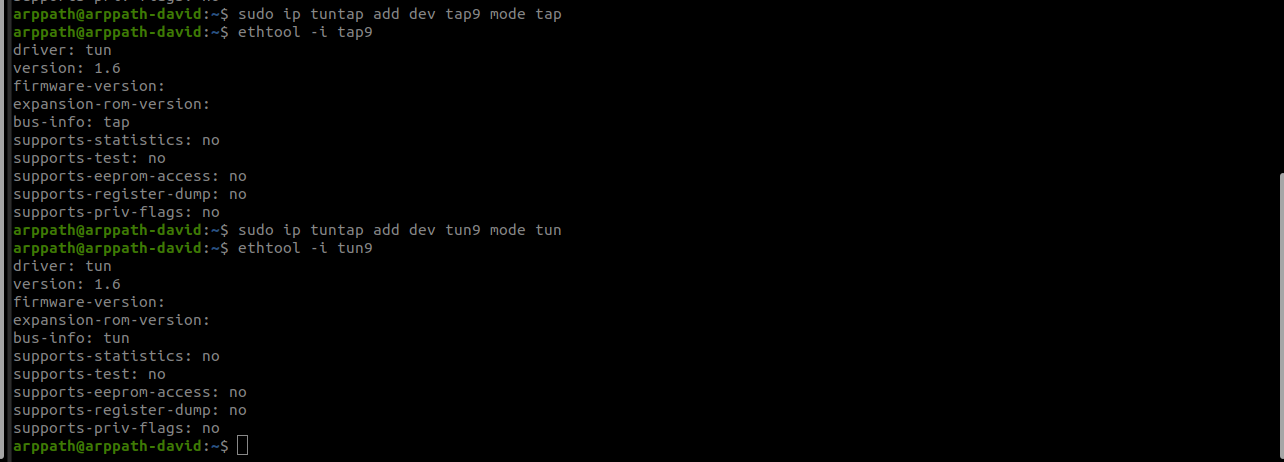
\includegraphics[width=\textwidth]{archivos/img/teoria/linux2.png}
    \caption{Comprobación con \texttt{ethtool} de tipo de interfaz virtual.}
    \label{fig:linux2}
\end{figure}


%%%%%%%%%%%%%%%%%%%%%%%%%%%%%%%%%%%%%%%%%%%%%%%%%%%%%%%%%%%%%%%%%%%%%%%%%%%%%%%%%%%%%%%%%%
\subsection{Interfaz virtual - \texttt{veth}}
\label{linuxVeths}
Las \gls{veth}, son interfaces de Ethernet virtuales creadas como un par de interfaces interconectadas entre si. El modelo funcional es sencillo, los paquetes enviados desde una son recibidos por la otra interfaz de forma directa, bastante parecido al funcionamiento de las \textit{pipes}. Una condición interesante de estas interfaces es que su gestión está asociada, es decir, si se levanta una extremo de la \gls{veth}, la otra también lo hará, si por el contrario se deshabilita o se destruye algún extremo de un par de \gls{veth} el otro extremo también se verá afectado \cite{veth}.\\
\par
Es muy común hacer uso de las \gls{veth} para interconectar \textit{Network Namespaces}, ya que, sabiendo que estas van a estar conectadas de forma directa, se puede utilizar este enlace como pasarela entre dos \textit{Network Namespaces}. De esta forma, se estaría interconectando dos \textit{stacks} independientes de red. La creación y destrucción de este tipo de interfaces se puede apreciar en el bloque \ref{code:iproute2_veth_use}, se recuerda que es necesario permisos de súper usuario.\\

\begin{lstlisting}[language= bash, style=Consola, caption={Manejo de Veths},label=code:iproute2_veth_use]
    # Crear un par veth
    ip link add {nombre_veth1} type veth peer name {nombre_veth2}
    
    # Si se elimina un extremo, el otro también lo hará
    ip link delete {nombre_veth}
    
\end{lstlisting}
\vspace{0.5cm}


%%%%%%%%%%%%%%%%%%%%%%%%%%%%%%%%%%%%%%%%%%%%%%%%%%%%%%%%%%%%%%%%%%%%%%%%%%%%%%%%%%%%%%%%%%

\subsection{Herramienta \texttt{TC}}


\gls{tc}, es un programa de espacio de usuario el cual es la pieza fundamental de la \gls{qos} en el Kernel de Linux. Muchas de sus funcionalidades se pueden resumir en cuatro puntos:

\begin{itemize}
    \item \textsc{SHAPING}
    \item \textsc{SCHEDULING}
    \item \textsc{POLICING}
    \item \textsc{DROPPING}
\end{itemize}

Según su \textit{man-page}\footnote{\url{https://man7.org/linux/man-pages/man8/tc.8.html}}, el procesamiento del trafico para conseguir dichas funcionalidades, se lleva a cabo con tres tipos de objetos: \textbf{qdiscs}, \textbf{classes} y \textbf{filters}.

\subsubsection{Qdiscs}

El objeto \gls{qdics}, disciplina de cola, es un concepto básico en el Networking de Linux que indica el orden en que los miembros de la cola, en este caso paquetes, se seleccionan para el servicio. Por ejemplo, en un momento dado puede que una herramienta de espacio de usuario requiera de transmitir un paquete, dicho paquete será entregado al \textit{stack} de red, llegando en última instancia a la interfaz de red por la cual va a ser transmitido. En ese momento el paquete se encontrará encolado en una cola de a la espera de ser trasnmitido, estas colas estarán regidas por un \gls{qdics}. El \gls{qdics} por defecto es un pfifo, es un puro \textit{first-in}, \textit{first-out} con limitación en el tamaño de cola en número de paquetes.


\subsubsection{Classes}

La clases se podrían ver como una sub-\gls{qdics} de una \gls{qdics}. Una clase puede contener a su vez otra clase, o más clases, pudiendo conformar sistemas de \gls{qos} en detalle, véase la figura \ref{fig:linuxNet_tc}. Cuando los paquetes son recibidos en una cola administrada por un \gls{qdics}, estos pueden ser encolados en base a las características del paquete en otras colas,  gestionadas por otras clases. Esto permite por ejemplo, priorizar el envío de datos de una aplicación sobre otra. Para ello, los paquetes de ambas aplicaciones se clasificarán en distintas clases, dándole más prioridad a una clase sobre la otra, asignándole más recursos de transmisión y recepción.

%foto
\begin{figure}[ht]
    \centering
    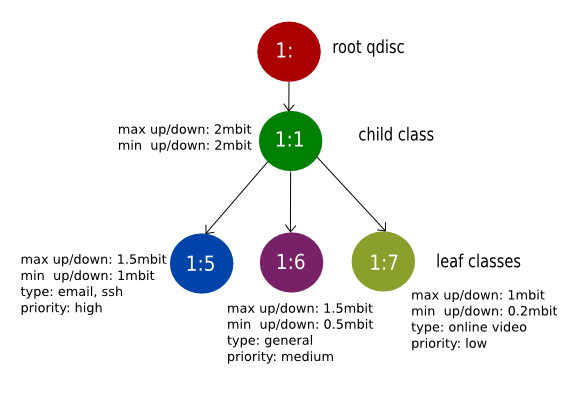
\includegraphics[width=8cm]{archivos/img/teoria/tc_qdisc_example_implementation.png}
    \caption{Sistema de QoS implementado con distintas clases \cite{qdiscs}}
    \label{fig:linuxNet_tc}
\end{figure}

\subsubsection{Filters}

Un filtro es usado para determinar con qué clase debe ser encolado el paquete. Para ello, el paquete siempre debe ser clasificado con una clase determinada. Varios tipos de filtros se pueden utilizar para clasificar los paquetes, pero en este caso será de interés el tipo de filtro \gls{bpf}\footnote{\url{https://man7.org/linux/man-pages/man8/tc-bpf.8.html}}, los cuales permiten anclar un \textit{bytecode} \gls{bpf}. Estos filtros se utilizarán para cargar programas \gls{bpf} que trabajarán en conjunto con \gls{xdp} con la finalidad de lograr el Broadcast. Esto es así, ya que en el \gls{tc} ya se hace uso de la estructura \texttt{sk\_buff} (Ir a \ref{linuxNetworking_skbuff}), por lo que ciertos \textit{helpers} \gls{bpf} para clonar paquetes podrán ser utilizados por \textit{bytecode} anclado en el filtro.


%%%%%%%%%%%%%%%%%%%%%%%%%%%%%%%%%%%%%%%%%%%%%%%%%%%%%%%%%%%%%%%%%%%%%%%%%%%%%%%%%%%%%%%%%%

\subsection{Namespaces}
\label{namespaces}
Una \textit{Namespace} se utiliza para aislar un recurso del sistema en una abstracción que hace  creer a los procesos dentro de dicha \textit{Namespace} que tienen su propia instancia del recurso en cuestión aislada del sistema real.  Los cambios realizados sobre recursos aislados del sistema, son solo visibles para procesos que son pertenecientes a la \textit{Namespace}, pero son invisibles para otros procesos pertenecientes al sistema o a otra \textit{Namespace}.\\
\par
Hay muchos tipos de \textit{Namespaces}, en la tabla \ref{tab:linux_ns} se pueden apreciar todos los tipos que existen a día de hoy. El uso de todos estos tipos de \textit{Namespaces} puede ser muy variado, pero el más importante de todos ellos son los contenedores. Los contenedores son elementos para correr aplicaciones, o herraminetas en un entorno aislado del sistema. A día de hoy, los contenedores más utilizados son los de Docker\footnote{\url{https://www.docker.com/}}, pero, ¿Realmente que hace Docker, qué es Docker?\\
\par

Docker se vale de las bondades del Kernel de Linux para aislar recursos y con esto conformar contenedores. Éste hará uso de las APIs suministradas por el Kernel para crear y destruir a conveniencia las distintas \textit{Namespaces}. Por lo que, Docker en verdad simplemente es un envoltorio de las llamadas al sistema para gestionar \textit{Namespaces}. Docker además, provee de distintos aspectos al usuario como \textit{copy-on-write}, o una configuración en modo \textit{bridge} hacia el exterior, pero en el fondo es
un mero \textit{wrapper} para la gestión de las \textit{Namespaces} con la finalidad de implementar contenedores.

% \begin{table}[ht]
%     \centering
%     \resizebox{\textwidth}{!}{%
%         \begin{tabular}{|l|l|}
%             \hline
%             \rowcolor[HTML]{EFEFEF}
%             \multicolumn{1}{|c|}{\cellcolor[HTML]{EFEFEF}{\color[HTML]{24292E} \textbf{Tipo de Namespace}}} & \multicolumn{1}{c|}{\cellcolor[HTML]{EFEFEF}{\color[HTML]{24292E} \textbf{Descripción}}}                                                                                                                                                     \\ \hline
%             \textbf{Cgroup}                                                                                 & \begin{tabular}[c]{@{}l@{}}Namespace utilizada generalmente para establecer unos limites de recursos,  por ejemplo, \\ CPU, memoria, lecturas y escrituras a disco, de todos los procesos que corran dentro de dicha Namespace.\end{tabular} \\ \hline
%             Time                                                                                            & Namespace para establecer una hora del sistema diferente a la del sistema.                                                                                                                                                                   \\ \hline
%             \textbf{Network}                                                                                & Namespace utilizada para tener una replica aislada del stack de red del sistema, dentro del propio sistema.                                                                                                                                  \\ \hline
%             \textbf{User}                                                                                   & Namespace utilizada para tener aislados a un grupo de usuarios.                                                                                                                                                                              \\ \hline
%             \textbf{PID}                                                                                    & Namespace utilizada para tener identificadores de proceso independientes de otras namespaces.                                                                                                                                                \\ \hline
%             \textbf{IPC}                                                                                    & Namespace utilizada para aislar los mecanismos de comunicación entre procesos.                                                                                                                                                               \\ \hline
%             \textbf{Uts}                                                                                    & Namespace utilizada para establecer un nombre de Host y nombre de dominio diferentes de los establecidos en el sistema                                                                                                                       \\ \hline
%             \textbf{Mount}                                                                                  & Namespace utilizada para aislar los puntos de montaje en el sistema de archivos.                                                                                                                                                             \\ \hline
%         \end{tabular}%
%     }
%     \caption{Resumen de los tipos de Namespaces en el Kernel de Linux}
%     \label{tab:linux_ns}
% \end{table}


\begin{table}[ht]
    \centering
    \resizebox{\textwidth}{!}{%
        \begin{tabular}{|l|l|}
            \hline
            \rowcolor[HTML]{EFEFEF}
            \multicolumn{1}{|c|}{\cellcolor[HTML]{EFEFEF}{\color[HTML]{24292E} \textbf{Tipo de Namespace}}} & \multicolumn{1}{c|}{\cellcolor[HTML]{EFEFEF}{\color[HTML]{24292E} \textbf{Descripción}}}                                                                                                                                   \\ \hline
            \textbf{Cgroup}                                                                                 & \begin{tabular}[c]{@{}l@{}}Namespace utilizado generalmente para establecer límites de recursos,\\ como CPU, memoria, lecturas y escrituras a disco, para todos los procesos\\ dentro de la misma Namespace. \end{tabular} \\ \hline
            Time                                                                                            & \begin{tabular}[c]{@{}l@{}}Namespace utilizado para establecer una hora del sistema diferente\\ a la del sistema global.\end{tabular}                                                                                      \\ \hline
            \textbf{Network}                                                                                & \begin{tabular}[c]{@{}l@{}}Namespace utilizado para crear una réplica aislada del stack de red \\ del sistema dentro del propio sistema.      \end{tabular}                                                                \\ \hline
            \textbf{User}                                                                                   & Namespace utilizado para aislar un grupo de usuarios.                                                                                                                                                                      \\ \hline
            \textbf{PID}                                                                                    & \begin{tabular}[c]{@{}l@{}}Namespace utilizado para tener identificadores de proceso independientes\\ de otras namespaces. \end{tabular}                                                                                   \\ \hline
            \textbf{IPC}                                                                                    & Namespace utilizado para aislar los mecanismos de comunicación entre procesos.                                                                                                                                             \\ \hline
            \textbf{Uts}                                                                                    & \begin{tabular}[c]{@{}l@{}}Namespace utilizado para establecer un nombre de host y nombre de dominio \\ diferentes de los establecidos en el sistema.      \end{tabular}                                                   \\ \hline
            \textbf{Mount}                                                                                  & Namespace utilizado para aislar los puntos de montaje en el sistema de archivos.                                                                                                                                           \\ \hline
        \end{tabular}%
    }
    \caption{Resumen de los tipos de Namespaces en el Kernel de Linux}
    \label{tab:linux_ns}
\end{table}


\subsubsection{Persistencia de las Namespaces}

Atendiendo a la \textit{man-page} \cite{ns} sobre \textit{Namespaces}, es importante señalar que las \textit{Namespaces} tienen una vida finita. La vida finita de la \textit{Namespace} dependerá de si la \textit{Namespace} en cuestión está referenciada, por lo que éstas vivirán siempre y cuando estén referenciadas, cuando dejen de estarlo serán destruidas.\\
\par
Este concepto de vida finita, será útil entenderlo para tener una mejor comprensión sobre el funcionamiento interno de Mininet ó Mininet-WiFI, los cuales se valen de estos conceptos para ahorrarse operaciones y ganar en rendimiento.  Una Namespace a día de hoy puede ser referenciada de tres maneras distintas:\\

\begin{itemize}
    \item Siempre y cuando haya un proceso corriendo dentro de esta \textit{Namespace}.
    \item Siempre que haya abierto un descriptor de archivo al fichero identificativo de la \textit{Namespace} (\texttt{/proc/{pid}/ns/{tipo\_namespace}}).
    \item Siempre que exista un \textit{bind-mount} del fichero (\texttt{/proc/{pid}/ns/{tipo\_namespace}}) de la \textit{Namespace} en cuestión.
\end{itemize}

Si ninguna de estas condiciones se cumple, la \textit{Namespace} en cuestión es eliminada automáticamente por el Kernel. Si se tratase de una \textit{Network Namespace}, aquellas interfaces que se encuentren en la \textit{Namespace} en desaparición volverán a la \textit{Network Namespace} por defecto \cite{ns}.

\subsubsection{Concepto de las Network Namespaces}

Una vez entendido el concepto de \textit{Namespace} en Linux, se introducen las \textit{Network Namespace}, las cuales serán fundamentales para las plataformas donde se probarán los distintos test. Éstas consisten en una replica lógica de \textit{stack} de red que por defecto tiene Linux, replicando rutas, tablas ARP, Iptables e interfaces de red \cite{netns}. \\
\par
Linux se inicia con un \textit{Network Namespace} por defecto, el espacio \textit{root}, con su tabla de rutas, su tabla ARP,  Iptables e interfaces de red. Pero también es posible crear más \textit{Network Namespace} no predeterminadas,  crear nuevos dispositivos en esos espacios de nombres, o mover un dispositivo existente de un espacio de nombres a otro. \\
\par
Para llevar todas estas tareas a cabo, la herramienta más sencilla será \texttt{iproute2} (Ir a Anexo \ref{iproute2}). Esta herramienta, haciendo uso del módulo \texttt{netns}, se podrá gestionar todo en lo relativo a las \textit{Network Namespace} con nombre. Esta coletilla, ``con nombre", atiende a que todas las \textit{Network Namespace} que se gestionen desde \texttt{iproute2} serán persistentes debido a que se realizará un \textit{bind-mount} con el nombre de la \textit{Namespace}, del fichero identificativo de la \textit{Namespace} en cuestión, bajo el directorio \texttt{/var/run/netns} . A continuación, se listan los comandos más frecuentes a la hora de gestionar \textit{Network Namespaces}, se entiende que se ejecutan con permisos de súper usuario.

\begin{lstlisting}[language= bash, style=Consola, caption={Comandos útiles con iproute2 - Netns},label=code:iproute2_ns_use]
    # Para crear una Network Namespace
    ip netns add {nombre netns}
    
    # Para listar las Network Namespaces "con nombre"
    ip netns list
    
    # Para añadir una interfaz a una Network Namespace
     ip netns set {nombre netns} Veth
    
    # Para ejecutar un comando dentro de una Network Namespace
    ip netns exec {nombre netns} {cmd}
    
    # Para eliminar una Network Namespace
    ip netns del {nombre netns}
    
\end{lstlisting}

\subsubsection{Métodos de comunicación inter-Namespaces: \glsentryshort{veth}}
\label{linuxVeths}
Las \gls{veth}, son interfaces de Ethernet virtuales creadas como un par de interfaces interconectadas entre si. El modelo funcional es sencillo, los paquetes enviados desde una son recibidos por la otra interfaz de forma directa, bastante parecido al funcionamiento de las \textit{pipes}. Una condición interesante de estas interfaces es que su gestión está asociada, es decir, si se levanta una extremo de la \gls{veth}, la otra también lo hará, si por el contrario se deshabilita o se destruye algún extremo de un par de \gls{veth} el otro extremo también se verá afectado \cite{veth}.\\
\par
Es muy común hacer uso de las \gls{veth} para interconectar \textit{Network Namespaces}, ya que, sabiendo que estas van a estar conectadas de forma directa, se puede utilizar este enlace como pasarela entre dos \textit{Network Namespaces}. De esta forma, se estaría interconectando dos \textit{stacks} independientes de red. La creación y destrucción de este tipo de interfaces se puede apreciar en el bloque \ref{code:iproute2_veth_use}, se recuerda que es necesario permisos de súper usuario.\\

\begin{lstlisting}[language= bash, style=Consola, caption={Manejo de Veths},label=code:iproute2_veth_use]
    # Crear un par veth
    ip link add {nombre_veth1} type veth peer name {nombre_veth2}
    
    # Si se elimina un extremo, el otro también lo hará
    ip link delete {nombre_veth}
    
\end{lstlisting}
\vspace{0.5cm}

Por lo tanto, se puede llegar al siguiente diagrama básico del funcionamiento de un par de \gls{veth}, las cuales estarán asignadas a una \textit{Network Namespace} distinta.  Como se puede apreciar en la figura \ref{fig:linuxNet_veth}, ambas interfaces están conectadas entre si directamente de forma interna en el propio Kernel. En el caso de que se generen paquetes desde una \textit{Network Namespace} hacia la otra, estos paquetes llegarán desde un extremo de la \gls{veth} directamente al otro extremo de la \gls{veth} a través del Kernel, y en este caso, la \textit{Network Namespace} por defecto no percibirá dicho trafico.\\
\par
Esta condición será de gran utilidad para recrear enlaces entre nodos independientes de red, los nodos se replicarán con \textit{Network Namespaces} y los enlaces con \gls{veth}s. Estos mecanismos serán utilizados por herramientas de emulación de redes como Mininet o Mininet-WiFI, más adelante se destallará.

\begin{figure}[ht]
    \centering
    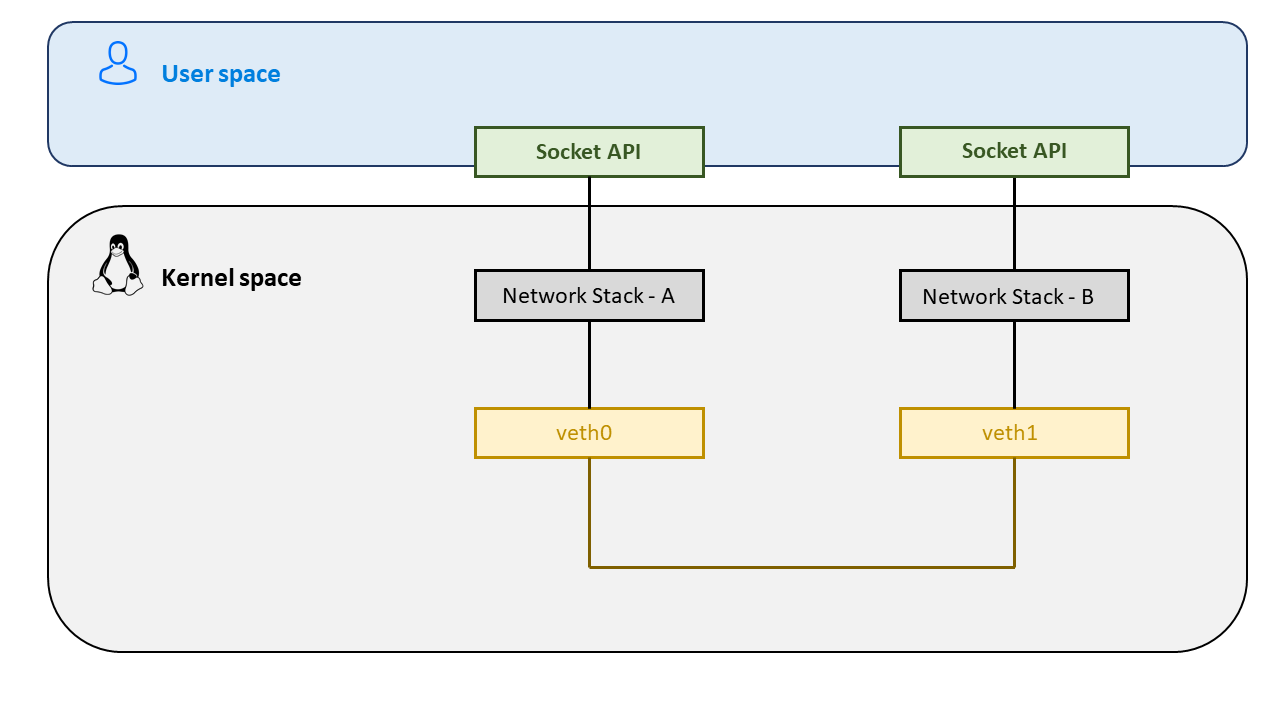
\includegraphics[width=15.5cm]{archivos/img/teoria/user_kernel.png}
    \caption{Enlace entre interfaces Veth separadas en dos Network Namespaces}
    \label{fig:linuxNet_veth}
\end{figure}